\documentclass[11pt,twoside,a4paper]{article}
\usepackage{fullpage}
\usepackage{graphicx}
\usepackage{amsmath}
\title{Wettbewerb Matrixoptik}
\author{Alain}

\begin{document}
	\maketitle
	\section{Analyse Aufgabenstellung}
	Ziel der Aufgabe ist, ein Optisches System aus vier bi-konvexen Linsen zu analysieren und mit Hilfe der Matrixoptik zu berechnen. \\
	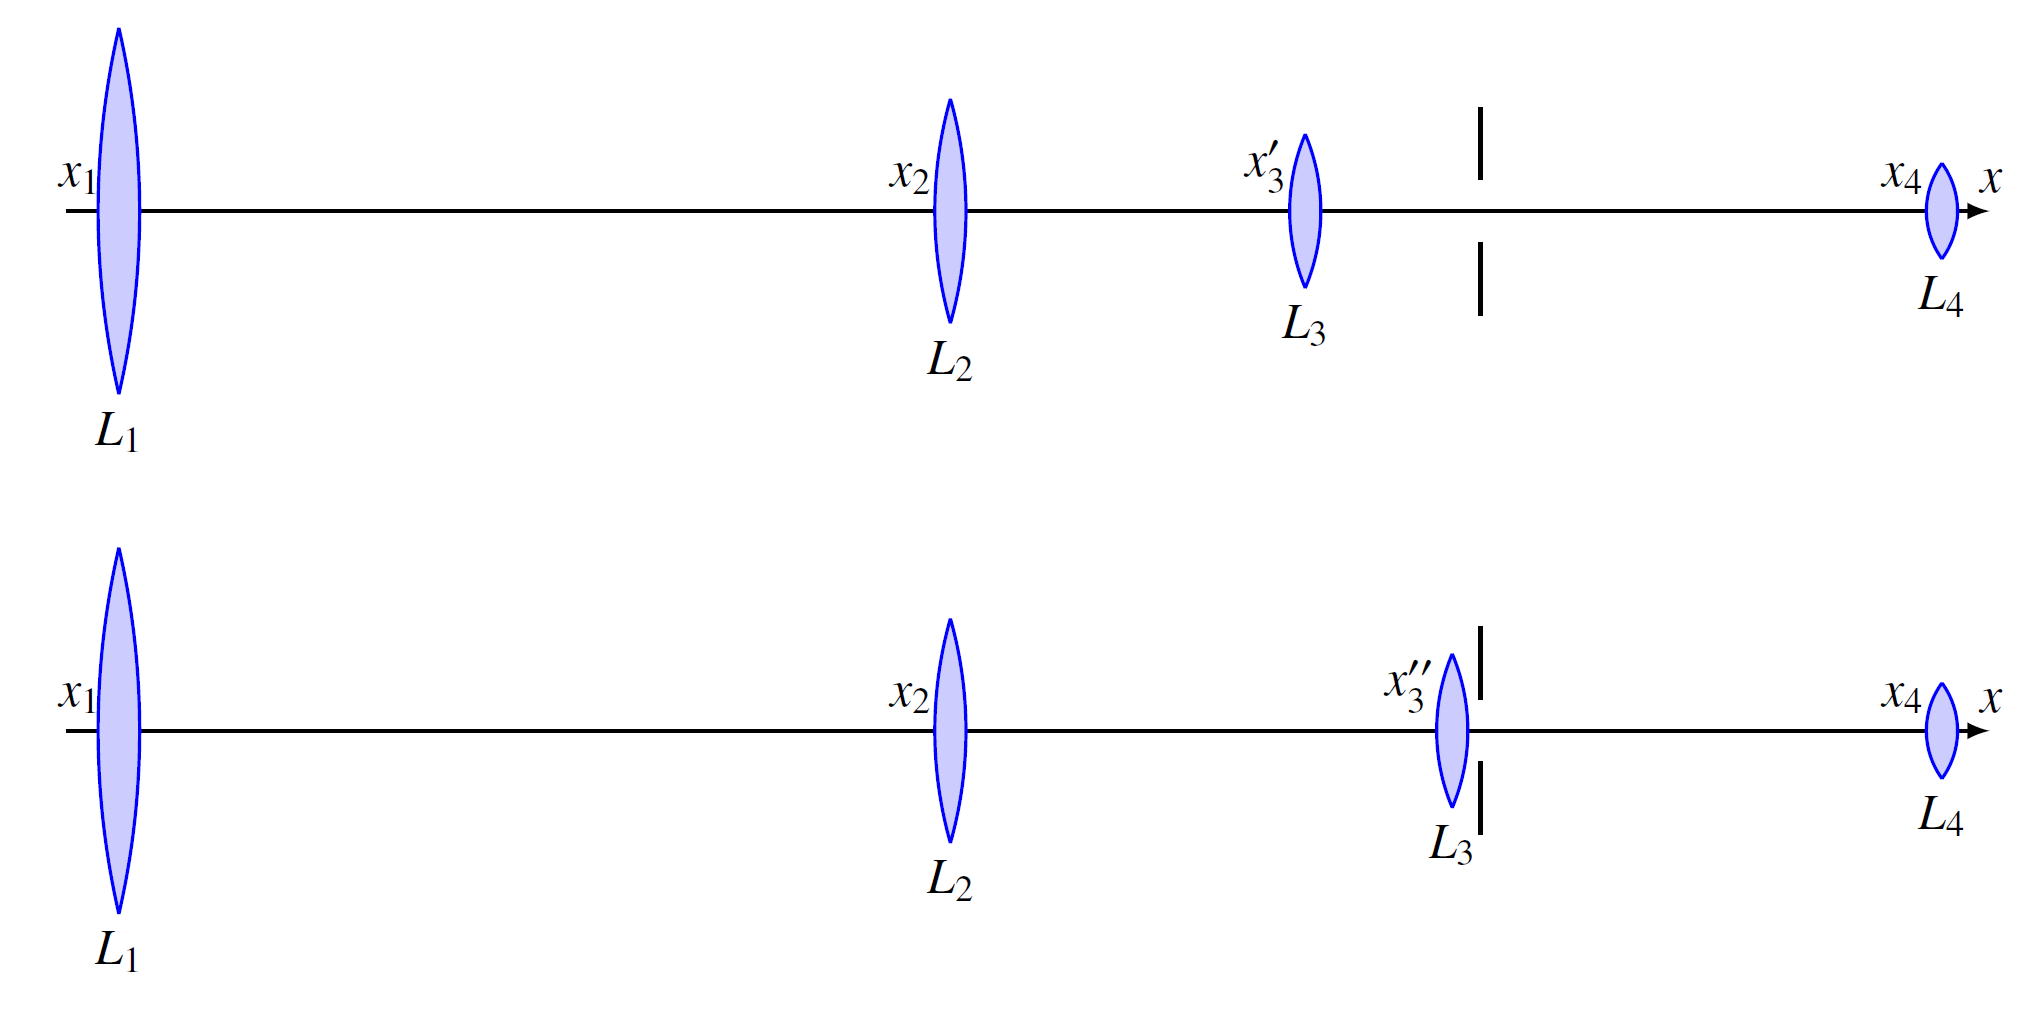
\includegraphics[scale=.25]{./system.PNG}
	\begin{table}
		\centering
		\begin{tabular}{lllll}
			Brechungsindex n & Linse & Krümmungsradius R [mm]& Dicke d [mm] & Position x [mm] \\
			1.5 & \(L_{1}\) & 78.672364 & 4 & \(x_{1}\) = 0 \\
			1.5 & \(L_{2}\) & 39.603940 & 3 & \(x_{2}\) = 80 \\
			1.5 & \(L_{3}\) & 19.013503 & 3 & \(x'_{3}\) = \(x_{2} + 20 * (1+\frac{1}{\sqrt{2}})\)  \\
			1.5 & \(L'_{3}\) & 19.013503 & 3 & \(x''_{3}\) = \(x_{2} + 20 * (1+\sqrt{2})\) \\
			1.5 & \(L_{4}\) & 7.8042263 & 3 & \(x_{4}\) = Unbekannt \\
		\end{tabular}
	\end{table} \\
	Das ganze Optische System, wie in der Darstellung dargestellt, mit den Daten der Tabelle 1 lässt sich mit Hilfe der Matrixoptik berechnen. Das Verhalten eines Lichtstrahles, welcher durch dieses Optische System geht, lässt sich mit einer Transfermatrix beschreiben. Durch diese Matrix lässt sich der Ausgangswinkel und -Höhe eines einfallenden Lichtstrahles mit bekanntem Einfallswinkel, und -Höhe berechnen. Da in dieser Aufgabe das System nur angenähert berechnet wird, wird mit \(sin(\theta) = \theta\) gerechnet.
	\begin{equation} \label{Transfermatrix1}
	\begin{pmatrix}
	A & B \\
	C & D
	\end{pmatrix}
	\quad
	\begin{pmatrix}
	y_{1}\\
	\theta_{1}
	\end{pmatrix}
	\quad
	=
	\quad
	\begin{pmatrix}
	y_{2}\\
	\theta_{2}
	\end{pmatrix}
	\end{equation}
	\ref{Transfermatrix1} Beispiel einer Transfermatrix multipliziert mit dem Lichtstrahl-Vektor wobei y die Höhe über der optischen Achse (x in der Abbildung) des Lichtstrahles und \(\theta\) den Winkel zur optischen Achse beschreibt \\
	
	Das Ziel ist es eine solche Transfermatrix dieses optischen Systems zu berechnen. 
	\section{Aufgabe 1}
	In dieser Aufgabe müssen wir die Position der letzten Linse \(L_{4}\) so berechnen, dass das System scharf abbildet. Dies ist, wie in der Aufgabenstellung schon beschrieben, der Fall wenn horizontal einfallende Strahlen wieder Horizontal austreten. Allgemein kann man sagen, dass eintretende Strahlen, welche zueinander parallel sind, wieder zueinander parallel austreten.
	Das bedeutet für die Transfermatrix, wenn ein Strahl mit \(\theta_{1} = 0\) und \(y_{1} \neq 0\) in das System kommt dieser wieder mit \(\theta_{2} = 0\) austritt. Anders ausgedrückt: 
	\begin{equation} \label{scharfAbb}
	\begin{aligned}[C]
		C * y_{1} + D * \theta_{1} = 0 \nonumber \\
		\textrm{Da \(\theta_{1} = 0\) und \(y_{1} \neq 0\) kann man vereinfachen:} \nonumber\\
		C = 0
	\end{aligned}
	\end{equation}
	Das heisst mit der Position C in der Transfermatrix können wir die gesuchte Position der Linse 4 berechnen. \\
	Damit wir die die oben genannte Rechnung durchführen können benötigen wir die Transfermatrix \(T\), berechnet mit der unbekannten \(x_{4}\).  
	\subsection{Berechnung von T}
	Die Transfermatrix des gesamten Systems besteht aus den jeweiligen Transfermatrizen der einzelnen Linsen und Räume zwischen den Linsen. Für jeden Raum, und Mediumswechsel, welcher ein Lichtstrahl durchquert gibt es eine Transfermatrix. In verkehrter Reihenfolge, wie sich der Lichtstrahl bewegt, multipliziert ergeben sie die Transfermatrix des gesamten Systems.
	\begin{equation} \label{tMatrixRaum}
	T_{l} = 
	\begin{pmatrix}
	1 & l \\
	0 & 1
	\end{pmatrix}
	\end{equation}
	\ref{tMatrixRaum} Matrix um einen Lichtstrahl, welcher sich durch einen Raum aus einem Medium bewegt, beschriebt. \(l\) ist die Länge dieses Raumes.
	\begin{equation} \label{tMatrixBrechung}
		B(n_{1},n_{2},R) = 
		\begin{pmatrix}
		1 & 0 \\
		\frac{1}{R}(\frac{n_{1}}{n_{2}}-1) & \frac{n_{1}}{n_{2}}
		\end{pmatrix}
	\end{equation}
	\ref{tMatrixBrechung} Transfermatrix um eine Brechung an einer gekrümmten Oberfläche zu berechnen. \(n_{1}\) ist der Brechungsindex des Mediums von dem der Lichtstrahl kommt und \(n_{2}\) derjenige des Mediums in das der Lichtstrahl geht. Der Radius R ist bei einem Übergang an einer konvexen Oberfläche positiv und bei einer konkaven negativ. Die Brechungsmatrix basiert auf dem Brechungsgesetz von Snellius.  \\
	Will man nun beschreiben wie sich ein Lichtstrahl durch eine Linse bewegt braucht man drei Transfermatrizen, die Brechung beim eintritt, wie sich der Strahl durch die Linse bewegt, und die Brechung beim Austritt. Die Transfermatrix erfolgt nun aus der Multiplikation dieser drei Matrizen. Für eine symmetrische bi-konvexe Linse sieht das wie folgt aus: 
	\begin{equation} \label{SymmLinse}
	B(n_{2},n_{1},-R)*T_{l}*B(n_{1},n_{2},R) = T
	\end{equation}
	Hat man nicht nur eine sondern zwei Linsen mit einem Abstand \(a\) dazwischen muss man diesen in die Rechnung miteinbeziehen. Die Rechnung würde dann wie folgt aussehen: 
	\begin{equation} \label{SymmLinse}
	T_{2}*T_{a}*T_{1} = T
	\end{equation}
	Auf das System der Aufgabe angewandt sieht die Berechnung der Transfermatrix so aus: 
	\begin{equation} \label{TLinsSys}
	T = T_{L4}T_{a3}T_{L3}T_{a2}T_{L2}T_{a1}T_{L1}
	\end{equation}
	\ref{TLinsSys} Die Matrizen \(T_{a1},T_{a2},T_{a3}\) beschrieben den Abstand zwischen den Linsen. Dabei ist zu beachten, dass bei \(T_{a3}\) die Distanz noch Unbekannt ist, und bei den bekannten Distanzen die Dicken der Linsen subtrahiert werden, um die Distanz zwischen den Linsenoberflächen zu erhalten. Die Matrizen \(T_{L1},T_{L2},T_{L3},T_{L4}\) beschrieben die Transfermatrizen der Linsen. Diese wurden nach dem oben erwähnten Prinzip berechnet, wobei für den Brechungsindex \(a_{1}\) 1 verwendet wurde, da in der Aufgabe die Linsen von Luft, für welches n = 1 gilt, umgeben sind.
\end{document}